
\subsection{Trip Generation}

We had to rely on the Gravity Model of transportation planning in
order to estimate the trip generation. However, we adjusted it to fit
our needs. Since the end point of all trips was the same, we did not
need the factor of $P_j$ and the model constant $K$ was just a
normalizing factor to make the total number of trips from all zones
equal to the total attendance. $K$ was calculated as
$(T_{ij}/T_{total}) \times (\mathrm{Total attendance})$. The map below
shows the results of the Gravity Model by displaying the number of
trips originating from each zip code to the stadium.

\begin{figure}[htp]
  \centering
  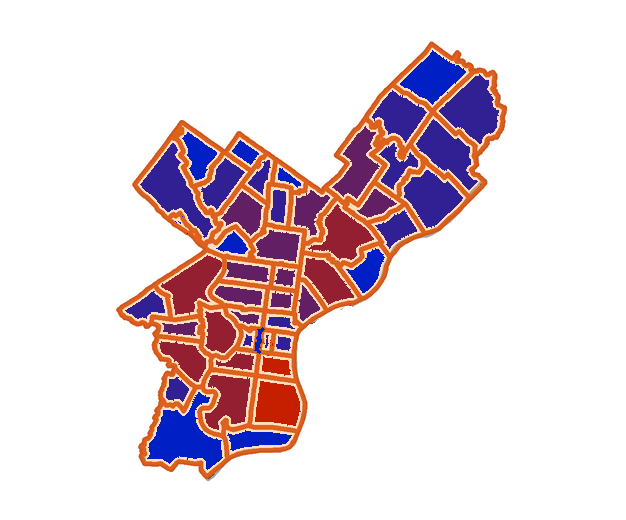
\includegraphics[height=8cm]{graphics/trip-generation.png}
  \caption{Map showing number of fans per zipcode}
  \label{fig-trip-generation-results}
\end{figure}

Looking at the results of the Gravity Model we can tell that ...

For more accuracy we could include more factors in the model such as
average income of the people living in the zone. We could also use
actual fan data, which we would need to obtain from the Phillies.


\subsection{Trip Distribution}

Trip Distribution data needs to be researched. The SEPTA website has a
Revenue and Ridership Report that gives trip distribution throughout
the day and also average daily ridership, which we can combine and
extrapolate to produce the average number of people riding per minute
throughout the day. Shown below is the trip distribution bar graph
provided in the February 2013 Revenue and Ridership Report:

\begin{figure}[htp]
  \centering
  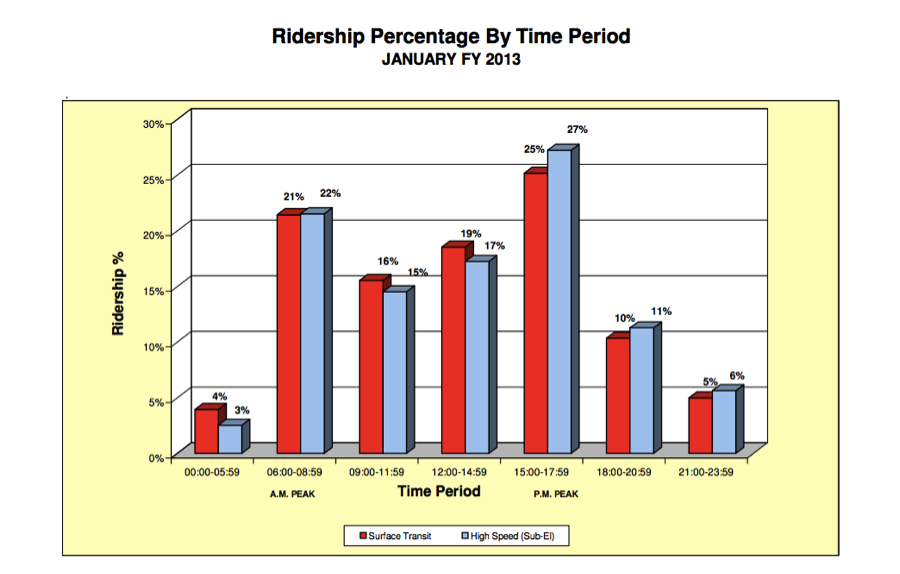
\includegraphics[height=7cm]{graphics/ridership-per-period.png}
  \caption{Average Daily Ridership By Time Period}
  \label{fig-ridership-per-period}
\end{figure}

Furthermore, we used data from a stadium planning study called Traffic
Operations Planning for Stadia and Arenas in order to obtain the
distribution of trips going to a stadium. Below is the table we
obtained:

\begin{table}
  \centering
  \begin{tabular}{cc}
    Minutes to Game Time & Percentage of Crowd \\
    \hline\hline
    -60 minutes & 24\% \\
    -40 minutes & 38\% \\
    -20 minutes & 54\% \\
     Game Time  & 72\% \\
    +20 minutes & 82\% \\
    +40 minutes & 92\% \\
    +60 minutes & 100\% \\
  \end{tabular}
  \caption{Cumulative arrivals to stadium as a percentage of total crowd (45,000 fans)}
  \label{tab-arrivals}
\end{table}

This table gives us the trip distribution for the trips that we
generated from the Trip Generation Gravity Model.


\subsection{Mode Choice}

As we had planned, we were able to obtain both parking lot data from
the Philadelphia Phillies, as well as average ridership data from
SEPTA. We found out that there were on average 7,400 trips per game on
SEPTA. Additionally, we found out there are typically 17,000 cars
parked in the parking lots every game. We found that if back-out the
average number of passengers per car we get 2, which has been
cross-referenced with traffic data for the United States. In order to
back out the number we assume 95\% occupancy of 43,651, or 41,468
total fans. We then removed the number of people taking SEPTA, which
gives us 34,068. Then divide that by the number of cars, which gives
us 2.


\subsection{Trip Assignment}

\subsubsection{SEPTA}

TBD

\subsubsection{Car-Micro}

TBD

\subsubsection{Car-Macro}

For the long Car model, we were able to utilize the Google Directions
API to retrieve both the distance and time from each zip code defined
in our model to the stadium. The results are stored as comma-separated
values that can be parsed easily from Python. The script needs to be
run two times for each zip code in a given set $Z$, which yields a
runtime of $O(|Z|)$, giving us the distance and time for both modes of
transportation, driving and transit.

Exhibit xx shows a table that provides a snippet of the zip code,
distance and time data when using transit to/from the stadium.

\begin{figure}[htp]
  \centering
  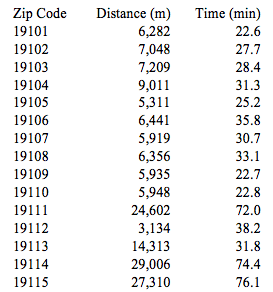
\includegraphics[height=8cm]{graphics/car-macro-ex.png}
  \caption{}
\end{figure}

\subsubsection{Transportation and GHG Results}

We were able to source accurate distance and time estimates (as stated
above) for fans traveling from each of the zip codes considered. Our
model then provided estimates for idling time based on congestion
levels and this led us to our first result making a direct comparison
between cars and SEPTA. We obtained was the distribution of travel
time across fans based on the trip generation model. We can see that
close to 12,000 people can save time traveling by SEPTA instead of
taking their car once we account for congestion and idling time in the
stadium. In fact, with only 20 minutes more, close to 40,000 fans can
switch from car to SEPTA, the benefits of which are displayed in our
second comparative result.

\begin{figure}[htp]
  \centering
  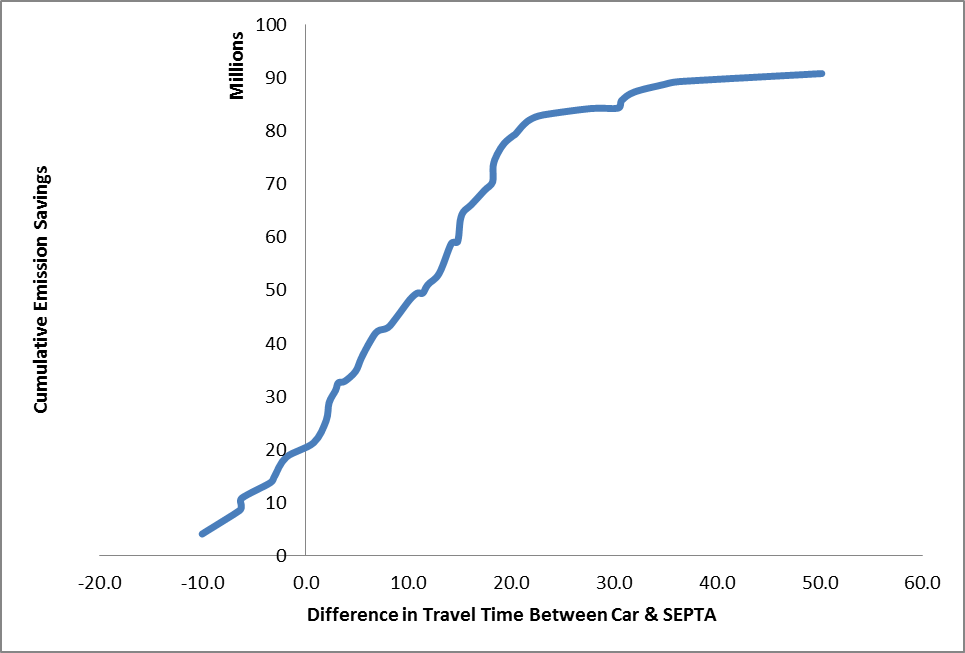
\includegraphics[height=8cm]{graphics/graph2.png}
  \caption{}
\end{figure}

We were able to establish accurate estimates for the average
greenhouse gas emissions for both gasoline and diesel cars. We also
sourced estimates for SEPTA train and bus emission per passenger mile
travelled. These estimates were used to compare the relative
environmental tradeoff of choosing cars over public transportation. We
can see that if the aforementioned 12,000 fans switch to SEPTA we
could cut down on approximately 20 million grams of CO2 per one-way
trip to or from a game. If the 40,000 fans identified above were to
switch, hypothetically, even after accounting for SEPTA capacity
constraints and waiting time, we would save close to 80 million grams
of CO2 per one-way trip.

\begin{figure}[htp]
  \centering
  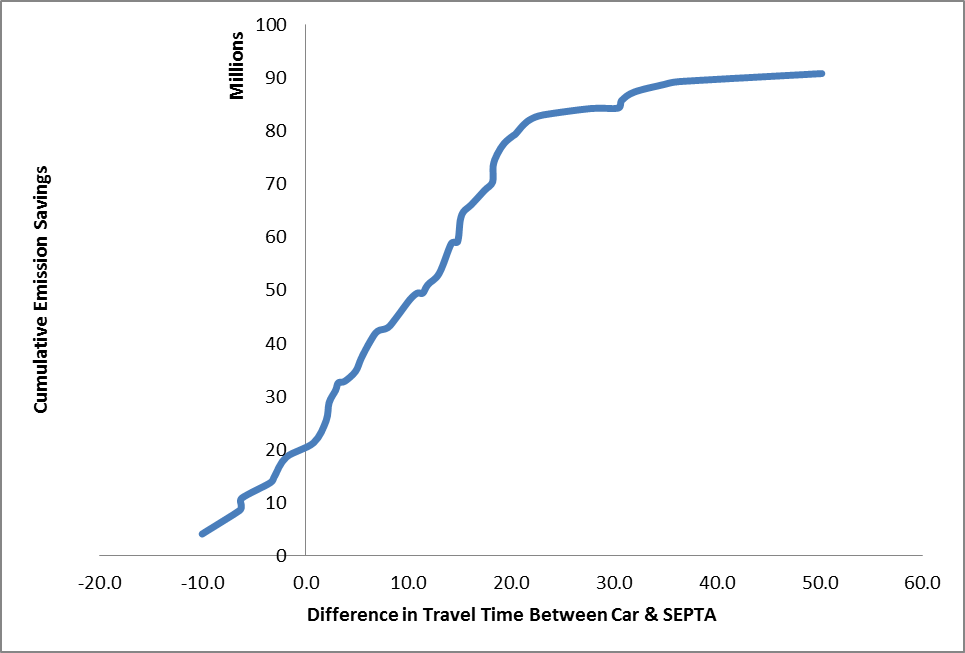
\includegraphics[height=8cm]{graphics/graph2.png}
  \caption{}
\end{figure}

\subsubsection{Output Results}

As specified in the design, the output was meant to be intuitive,
accessible and impactful. The options we considered were:

\begin{itemize}
    \item Mobile App (iOS, Android, Windows Phone)
    \item Web Application
    \item Desktop Application
\end{itemize}

The design that was settled upon was the second one, Web Application.

Mobile applications have the advantage of being very convenient but
the drawback is that proficiency required across multiple platforms
and programming languages as well as dealing with fragmentation across
versions of mobile operating systems (especially Android) is
especially difficult. Desktop applications suffer from rigidity in
that they are difficult to update on-the-fly and often require tedious
updates via desktop operating systems. As a result, web applications
provide the perfect balance for our project, allowing for updates as
well as accessibility from both desktops and mobile devices.

Once the form of output was finalized, further research was performed
to ensure that we satisfied our goal of having an ``intuitive''
output. Brainstorming was conducted with potential users of the web
application in order to determine the best layout for the information
to be displayed. Basic feedback was also obtained on the overall
aesthetic of the web application. Our basic implementation of the web
application was divided into five pages hosted on a local Python
simple server utilizing CGI scripts to serve webpages in response to
user input.

\begin{description}
    \item[Introduction Page] The introduction page serves as a landing
  page for users of our web application. There is an emission
  calculator, which takes as an input the user's address, zip code and
  vehicle miles per gallon as well as fuel type (gasoline or
  diesel). The page also displays the date and time of the next home
  page as well as the weather within one hour of the start of the game
  in order to allow users to make a more informed decision when
  selecting transportation. Finally, the page provides an overview of
  how the web application works and how emissions are calculated by
  our model.
  \begin{figure}[htp]
    \centering
    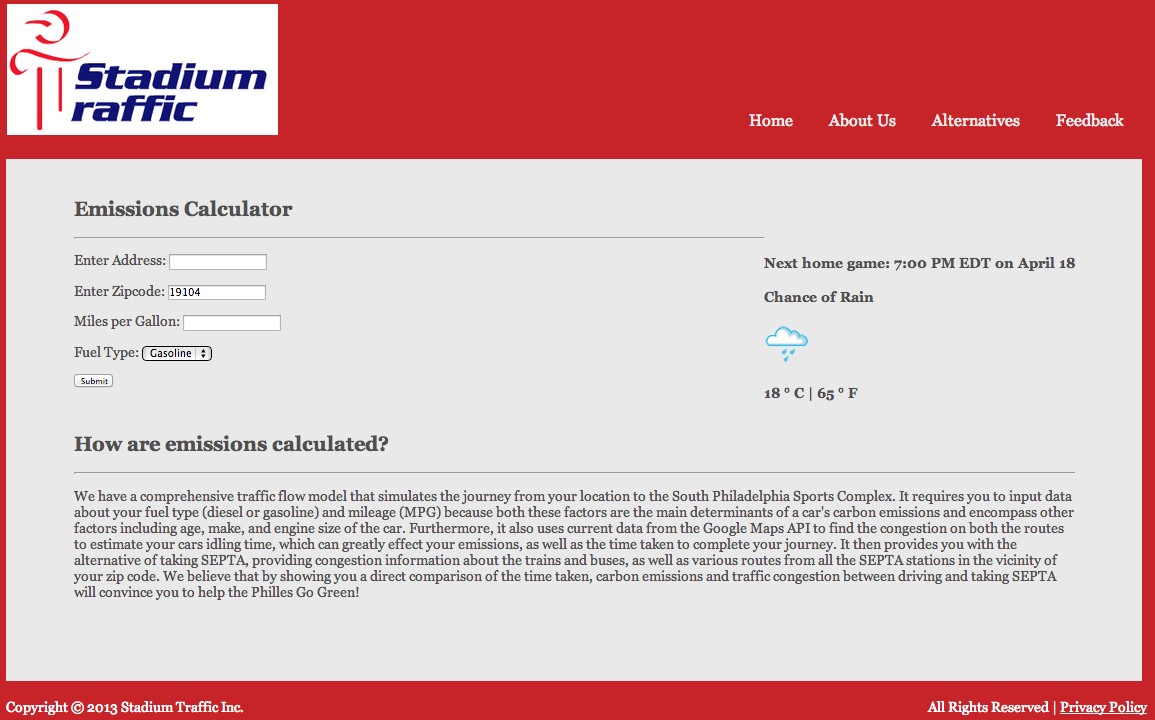
\includegraphics[height=8cm]{graphics/website/intro.png}
    \caption{}
  \end{figure}

    \item[Results Page] The results page is served when the ``submit''
  button on the introduction page is clicked with valid information in
  the form. The results page displays a Google Map showing driving
  directions from the origin to the stadium and provides a drop-down
  to switch to transit directions. The page also provides a
  comparative table between Car and Septa across four factors: time
  taken, distance, carbon emissions and congestion levels. The results
  in the table are driven by the model that we created and serve as
  the main ``output'' of our project.
  \begin{figure}[htp]
    \centering
    \begin{subfigure}{.4\textwidth}
      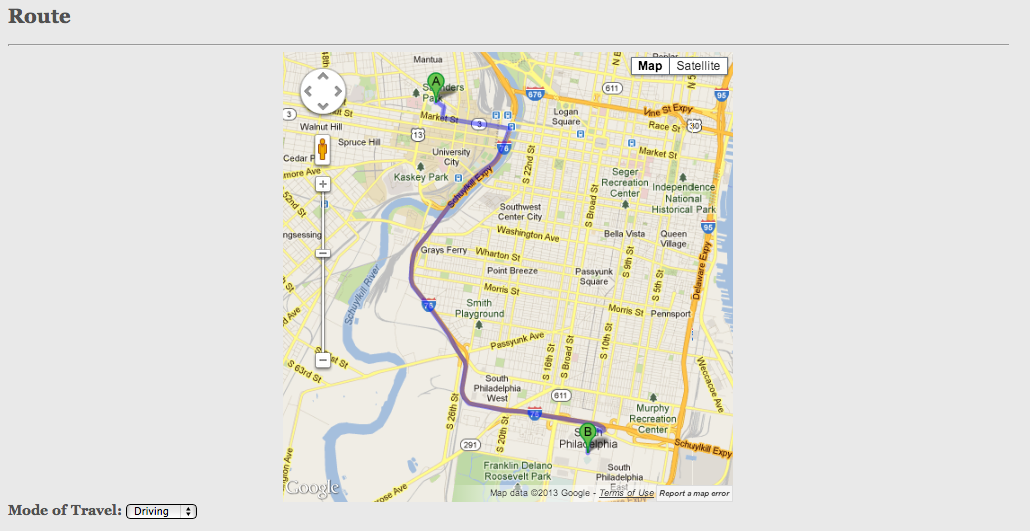
\includegraphics[height=8cm]{graphics/website/results-map.png}
      \caption{}
    \end{subfigure}
    \begin{subfigure}{.4\textwidth}
      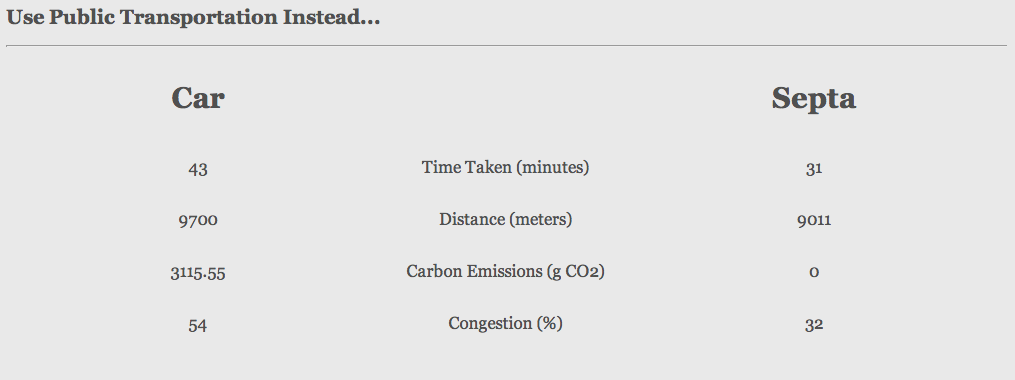
\includegraphics[height=8cm]{graphics/website/results-table.png}
      \caption{}
    \end{subfigure}
  \end{figure}

    \item[Alternatives Page] There might be users, however, who prefer
  not to switch to SEPTA. Given that our overall goal was to reduce
  carbon emissions from fans traveling to and from games, we suggest
  two alternatives that fans that utilize to cut down on their carbon
  emissions even if they do opt to take a car to the game. The first
  is to purchase carbon credits from a third-party vendor and the
  other is to utilize a public forum to find other fans to carpool
  with to the next home game.

  \begin{figure}[htp]
    \centering
    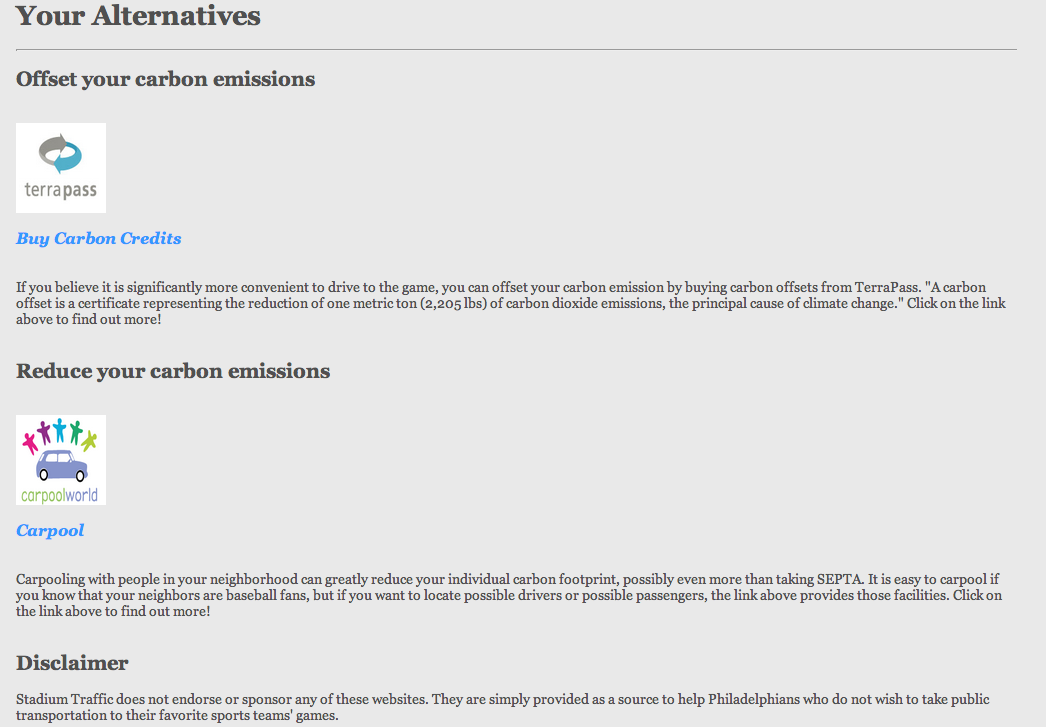
\includegraphics[height=8cm]{graphics/website/alternatives.png}
    \caption{}
  \end{figure}

    \item[About Page] The about page provides users with information
  about the motivations behind our project and a brief biography for
  each of the three members on our team.

  \begin{figure}[htp]
    \centering
    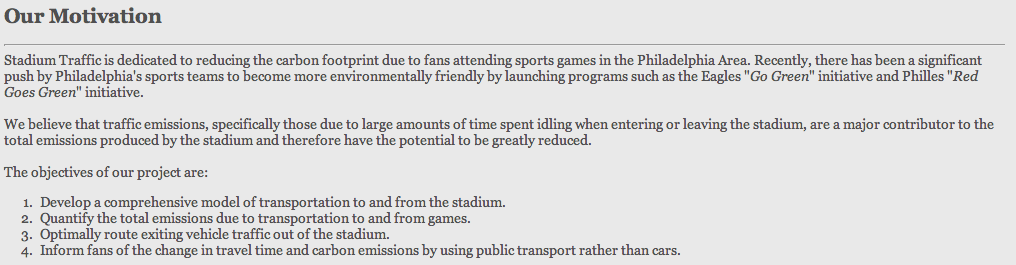
\includegraphics[height=8cm]{graphics/website/motivation.png}
    \caption{}
  \end{figure}

    \item[Feedback Page] The feedback page features a simple form that
  users can utilize to convey compliments/complaints to the Stadium
  Traffic team.

  \begin{figure}[htp]
    \centering
    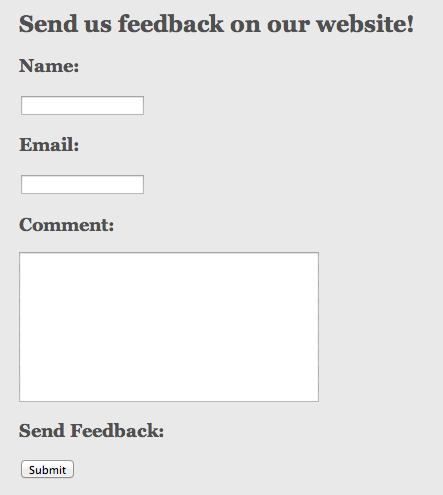
\includegraphics[height=8cm]{graphics/website/feedback.png}
    \caption{}
  \end{figure}
\end{description}

Also, our website contains a privacy policy that was added in order to
inform users about how the information they input will be stored and
utilized as is conventional in most web applications today.
